\section{Solution}
\label{sec:Solution}

In order to pursue the goal of introducing contracts to BDD, we introduce the Salad Framework. Salad contains three DSLs --- each with a specific purpose.

Gherkin is the BDD feature specification language, Lettuce is the transformation language and lastly, Tomato is a simplified version of JML.  Combined, they make it possible for contracts to be generated from feature descriptions and transformed into JML. Figure \ref{fig:saladoverview} illustrates the workflow from input to output.

\begin{figure}
  \begin{center}
    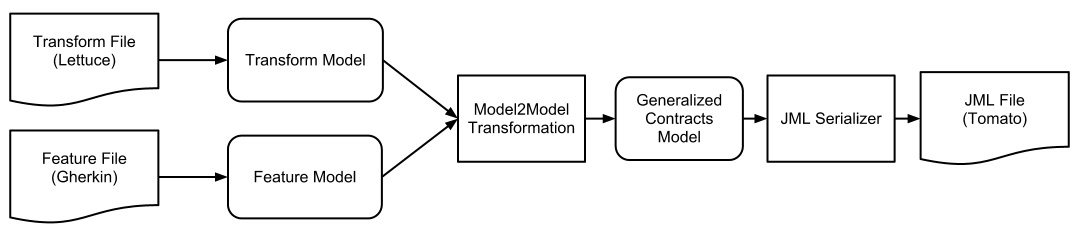
\includegraphics[scale=0.32]{images/framework_overview.png}
  \end{center}
  \caption{Salad Framework Overview}
  \label{fig:saladoverview}
\end{figure}

The Feature Model represents our extension of the feature language.
As a goal, we aim to provide extensions that allow current users of BDD to use
our language without much training.

Lettuce specifies how behaviors can be transformed into code contracts.
By specifying rules on how contracts are interpreted, the user decides the translation semantics of the natural language which represents the contracts. 

Through model-to-model transformation, the feature model(s) and the transform model(s) are transformed into a generalized contracted software model representing contracts describing the pre- and postconditions. 

These models can then be run through a specialized serializer, in our case the Tomato formatter which can generate JML files.
The textual representation of our JML model resembles Java syntax with classes containing methods and their contracts written in JML. 

\subsection{A Generalized Model for Contracted Software}
\label{sub:AGeneralizedModelforContractedSoftware}

In order to make our framework modularized and support multiple output programming languages, we have designed a generalized model which
we can make transformations to (see Figure~\ref{fig:generaloutputmodel}).

\begin{figure}
  \begin{center}
    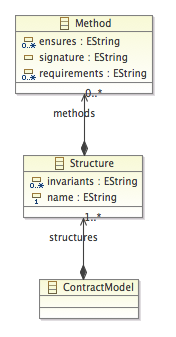
\includegraphics[scale=0.35]{images/generalized_outputmodel.png}
  \end{center}
  \caption{A General Model for Representing Contracted Software Systems}
  \label{fig:generaloutputmodel}
\end{figure}

The model consists of a number of structures, e.g. classes or interfaces, that contain a number of methods.
In the model we support the most common contracting features, namely preconditions, postconditions and invariants.

% Insert sentences about contracted model
